The next step was to investigate the pluggable circuit board, the process and results of which are discussed in this section.

\subsection{Circuit board macroanalysis}
The circuit board itself was identified as a product of AMD, housing a 500 MHz AMD Geode LX800 and 256 MB DDR DRAM (Figure~\ref{fig:circuit-board}). Such technology was not believed to exist at the time, and it seems that great efforts have been devoted to keep this technology hidden.


\begin{figure}[h]
	\centering
	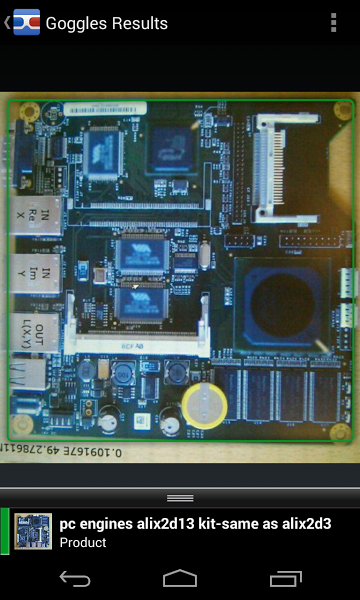
\includegraphics[width=0.8\columnwidth]{img/circuit-board.png}
	\caption{The identified circuit board}
	\label{fig:circuit-board}
\end{figure}

This leaves investigating yet another set of geographic coordinates: $0.109167E \; 49.278611N$. Learning from their previous experience, the geographic team decided to book a flight this time. They, of course, did not learn from their \emph{other} mistake, and hence spent quite some time travelling instead of taking the more sensible option of employing a parallel depth first search on the earth's map. The fact was reflected appropriately in their performance review. But we digress \ldots

\begin{figure}[h]
	\centering
	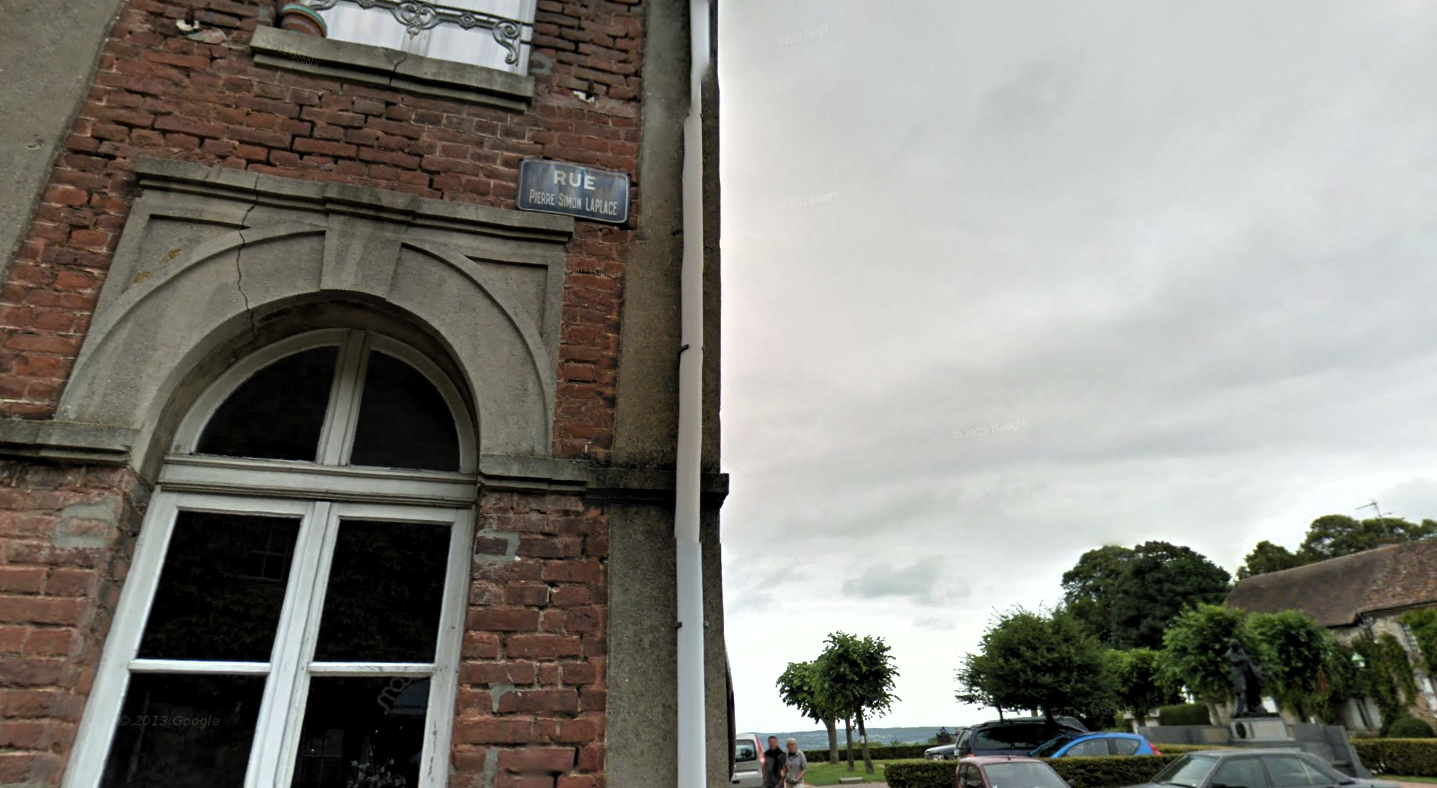
\includegraphics[width=0.95\columnwidth]{img/laplace-road.png}
	\caption{Rue Pierre Simon Laplace Road - You will never find a more blessed hive of charm and harmony}
	\label{fig:laplace-road}
\end{figure}


After an expensive trip to France, it was determined that the site referred to``Ecole Beaumont en auge'' at``Rue Pierre Simon Laplace Road'' (Figure~\ref{fig:laplace-road}). The connection was made the following week, when the team realised that the circuit was meant to employ some form of Laplace transform.


\subsection{Circuit board microanalysis}
